\newpage

\colorlet{cluster1}{blue!25}
\colorlet{cluster2}{gray}
\definecolor{cluster3}{rgb}{0.88,1,1}
\colorlet{cluster4}{red!25}
\begin{table}[h]
    \begin{center}
      \caption{Histograma - Resultado do conjunto lentilha em 4 grupos.}
\begin{tabular}{ |>{\centering\arraybackslash}m{4.9cm} | >{\centering\arraybackslash}m{4.9cm} | >{\centering\arraybackslash}m{4.9cm} | } 
	\hline
	\cellcolor{cluster1}
   \grbox{
   \begin{subfigure}[b]{5cm}
   \centering
   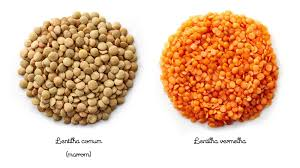
\includegraphics[width=5cm,height=2cm,keepaspectratio,trim=0 0 0 -5]{images/lentilha/0.jpeg} 
	\end{subfigure}}{0}
   &
   \cellcolor{cluster1}
    \grbox{
   \begin{subfigure}[b]{5cm}
  \centering
   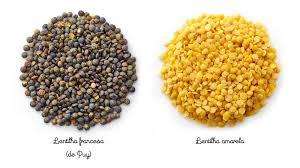
\includegraphics[width=5cm,height=2cm,keepaspectratio,trim=0 0 0 -5]{images/lentilha/5.jpeg} 
	\end{subfigure}}{5}
   & 
   \cellcolor{cluster1}
    \grbox{
   \begin{subfigure}[b]{5cm}
  \centering
   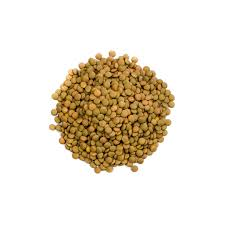
\includegraphics[width=5cm,height=2cm,keepaspectratio,trim=0 0 0 -5]{images/lentilha/18.jpeg} 
	\end{subfigure}}{18}
   \\ 
 
 \cellcolor{cluster1}
   \grbox{
   \begin{subfigure}[b]{5cm}
  \centering
   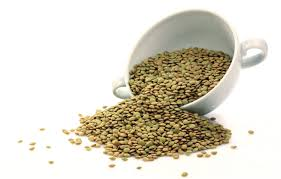
\includegraphics[width=5cm,height=2cm,keepaspectratio,trim=0 0 0 -5]{images/lentilha/28.jpeg} 
	\end{subfigure}}{28}
   &
   \cellcolor{cluster1}
   \grbox{
   \begin{subfigure}[b]{5cm}
  \centering
   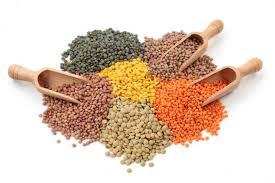
\includegraphics[width=5cm,height=2cm,keepaspectratio,trim=0 0 0 -5]{images/lentilha/30.jpeg} 
	\end{subfigure}}{\underline{30}}
   & 
   \cellcolor{cluster1}
   \grbox{
   \begin{subfigure}[b]{5cm}
  \centering
    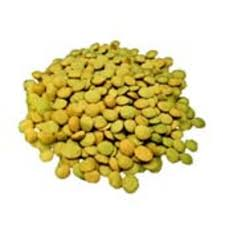
\includegraphics[width=5cm,height=2cm,keepaspectratio,trim=0 0 0 -5]{images/lentilha/31.jpeg} 
	\end{subfigure}}{31}
   \\ 
   \cellcolor{cluster1}
   \grbox{
   \begin{subfigure}[b]{5cm}
  \centering
   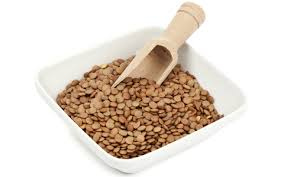
\includegraphics[width=5cm,height=2cm,keepaspectratio,trim=0 0 0 -5]{images/lentilha/32.jpeg} 
	\end{subfigure}}{32}
   &
   \cellcolor{cluster2}
   \grbox{
   \begin{subfigure}[b]{5cm}
  \centering
   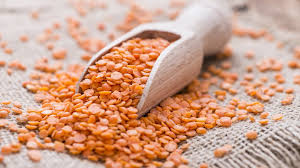
\includegraphics[width=5cm,height=2cm,keepaspectratio,trim=0 0 0 -5]{images/lentilha/12.jpeg} 
	\end{subfigure}}{12}
   & 
   \cellcolor{cluster2}
   \grbox{
   \begin{subfigure}[b]{5cm}
  \centering
    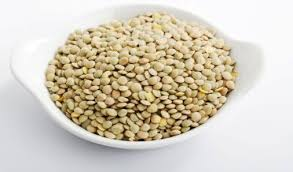
\includegraphics[width=5cm,height=2cm,keepaspectratio,trim=0 0 0 -5]{images/lentilha/15.jpeg} 
	\end{subfigure}}{15}
   \\ 
   
   \cellcolor{cluster2}
   \grbox{
   \begin{subfigure}[b]{5cm}
  \centering
   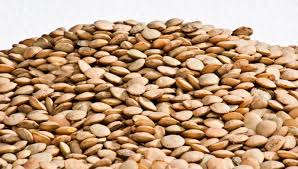
\includegraphics[width=5cm,height=2cm,keepaspectratio,trim=0 0 0 -5]{images/lentilha/24.jpeg} 
	\end{subfigure}}{\underline{24}}
   &
   \cellcolor{cluster3}
   \grbox{
   \begin{subfigure}[b]{5cm}
  \centering
   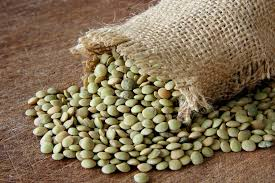
\includegraphics[width=5cm,height=2cm,keepaspectratio,trim=0 0 0 -5]{images/lentilha/9.jpeg} 
	\end{subfigure}}{9}
   & 
   \cellcolor{cluster3}
   \grbox{
   \begin{subfigure}[b]{5cm}
  \centering
    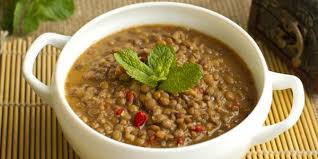
\includegraphics[width=5cm,height=2cm,keepaspectratio,trim=0 0 0 -5]{images/lentilha/11.jpeg} 
	\end{subfigure}}{11}
   \\ 
   
   \cellcolor{cluster3}
   \grbox{
   \begin{subfigure}[b]{5cm}
  \centering
   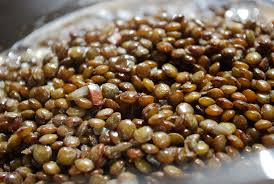
\includegraphics[width=5cm,height=2cm,keepaspectratio,trim=0 0 0 -5]{images/lentilha/10.jpeg} 
	\end{subfigure}}{10}
   &
   \cellcolor{cluster3}
   \grbox{
   \begin{subfigure}[b]{5cm}
  \centering
   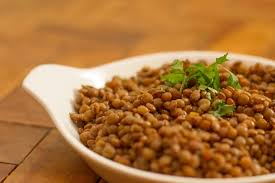
\includegraphics[width=5cm,height=2cm,keepaspectratio,trim=0 0 0 -5]{images/lentilha/14.jpeg} 
	\end{subfigure}}{14}   
   & 
   \cellcolor{cluster3}
   \grbox{
   \begin{subfigure}[b]{5cm}
  \centering
    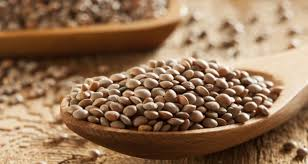
\includegraphics[width=5cm,height=2cm,keepaspectratio,trim=0 0 0 -5]{images/lentilha/1.jpeg} 
	\end{subfigure}}{1}    
   \\ 
   
   \cellcolor{cluster3}
   \grbox{
   \begin{subfigure}[b]{5cm}
  \centering
   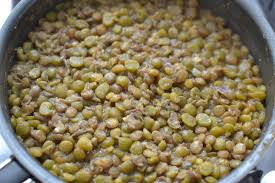
\includegraphics[width=5cm,height=2cm,keepaspectratio,trim=0 0 0 -5]{images/lentilha/16.jpeg} 
	\end{subfigure}}{16} 
   &
   \cellcolor{cluster3}
   \grbox{
   \begin{subfigure}[b]{5cm}
  \centering
   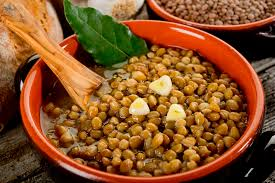
\includegraphics[width=5cm,height=2cm,keepaspectratio,trim=0 0 0 -5]{images/lentilha/17.jpeg} 
	\end{subfigure}}{17}
   & 
   \cellcolor{cluster3}
   \grbox{
   \begin{subfigure}[b]{5cm}
  \centering
    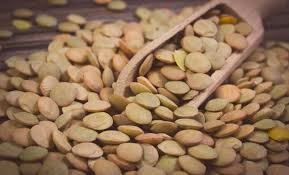
\includegraphics[width=5cm,height=2cm,keepaspectratio,trim=0 0 0 -5]{images/lentilha/20.jpeg} 
	\end{subfigure}}{20}
   \\ 
   
   \cellcolor{cluster3}
   \grbox{
   \begin{subfigure}[b]{5cm}
  \centering
   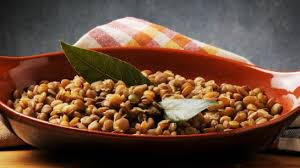
\includegraphics[width=5cm,height=2cm,keepaspectratio,trim=0 0 0 -5]{images/lentilha/21.jpeg} 
	\end{subfigure}}{21}
   &
   \cellcolor{cluster3}
   \grbox{
   \begin{subfigure}[b]{5cm}
  \centering
   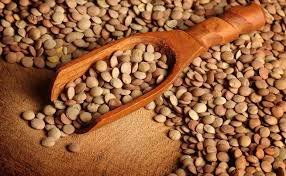
\includegraphics[width=5cm,height=2cm,keepaspectratio,trim=0 0 0 -5]{images/lentilha/26.jpeg} 
	\end{subfigure}}{\underline{26}}
   & 
   \cellcolor{cluster3}
   \grbox{
   \begin{subfigure}[b]{5cm}
  \centering
    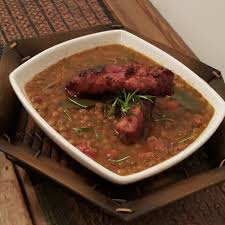
\includegraphics[width=5cm,height=2cm,keepaspectratio,trim=0 0 0 -5]{images/lentilha/27.jpeg} 
	\end{subfigure}}{27}
   \\ 
   
   \cellcolor{cluster3}
   \grbox{
   \begin{subfigure}[b]{5cm}
  \centering
   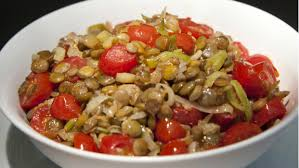
\includegraphics[width=5cm,height=2cm,keepaspectratio,trim=0 0 0 -5]{images/lentilha/29.jpeg} 
	\end{subfigure}}{29}
   &
   \cellcolor{cluster4}
   \grbox{
   \begin{subfigure}[b]{5cm}
  \centering
   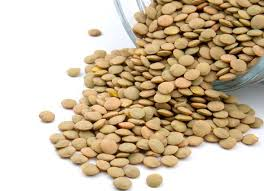
\includegraphics[width=5cm,height=2cm,keepaspectratio,trim=0 0 0 -5]{images/lentilha/3.jpeg} 
	\end{subfigure}}{3}
   & 
   \cellcolor{cluster4}
   \grbox{
   \begin{subfigure}[b]{5cm}
  \centering
    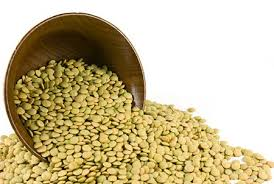
\includegraphics[width=5cm,height=2cm,keepaspectratio,trim=0 0 0 -5]{images/lentilha/4.jpeg} 
	\end{subfigure}}{4}
   \\
 
 \cellcolor{cluster4}
 \grbox{
   \begin{subfigure}[b]{5cm}
  \centering
   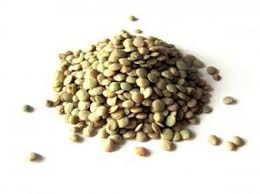
\includegraphics[width=5cm,height=2cm,keepaspectratio,trim=0 0 0 -5]{images/lentilha/19.jpeg} 
	\end{subfigure}}{19}
   &
   \cellcolor{cluster4}
   \grbox{
   \begin{subfigure}[b]{5cm}
  \centering
   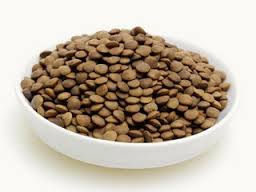
\includegraphics[width=5cm,height=2cm,keepaspectratio,trim=0 0 0 -5]{images/lentilha/13.jpeg} 
	\end{subfigure}}{13}
   & 
   \cellcolor{cluster4}
   \grbox{
   \begin{subfigure}[b]{5cm}
  \centering
    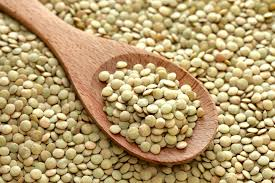
\includegraphics[width=5cm,height=2cm,keepaspectratio,trim=0 0 0 -5]{images/lentilha/2.jpeg} 
	\end{subfigure}}{2}
   \\
  \cellcolor{cluster4}
 \grbox{
   \begin{subfigure}[b]{5cm}
  \centering
   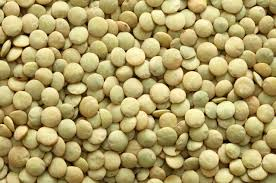
\includegraphics[width=5cm,height=2cm,keepaspectratio,trim=0 0 0 -5]{images/lentilha/6.jpeg} 
	\end{subfigure}}{6}
   &
   \cellcolor{cluster4}
   \grbox{
   \begin{subfigure}[b]{5cm}
  \centering
   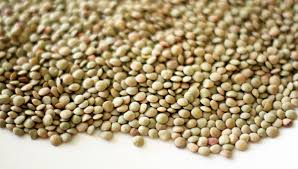
\includegraphics[width=5cm,height=2cm,keepaspectratio,trim=0 0 0 -5]{images/lentilha/7.jpeg} 
	\end{subfigure}}{\underline{7}}
   & 
   \cellcolor{cluster4}
   \grbox{
   \begin{subfigure}[b]{5cm}
  \centering
    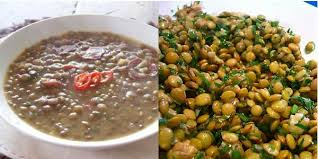
\includegraphics[width=5cm,height=2cm,keepaspectratio,trim=0 0 0 -5]{images/lentilha/8.jpeg} 
	\end{subfigure}}{8}
   \\
 \cellcolor{cluster4}
 \grbox{
   \begin{subfigure}[b]{5cm}
  \centering
   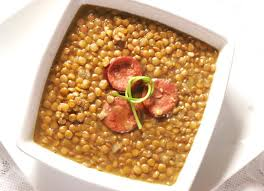
\includegraphics[width=5cm,height=2cm,keepaspectratio,trim=0 0 0 -5]{images/lentilha/22.jpeg} 
	\end{subfigure}}{22}
   &
   \cellcolor{cluster4}
   \grbox{
   \begin{subfigure}[b]{5cm}
  \centering
   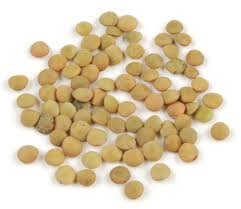
\includegraphics[width=5cm,height=2cm,keepaspectratio,trim=0 0 0 -5]{images/lentilha/23.jpeg} 
	\end{subfigure}}{23}
   &
   \cellcolor{cluster4}
   \grbox{
   \begin{subfigure}[b]{5cm}
  \centering
   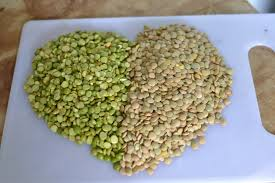
\includegraphics[width=5cm,height=2cm,keepaspectratio,trim=0 0 0 -5]{images/lentilha/25.jpeg} 
	\end{subfigure}}{25}
    \\
  \hline
\end{tabular}
\label{lentilhaHistograma}
\legend{\textbf{Fonte:} \citeonline{google3}.}
\end{center}
\end{table}